\documentclass[11pt,a4paper]{article}
\usepackage{acl}
\usepackage{times}
\usepackage{latexsym}
\usepackage{booktabs}
\usepackage{multirow}
\usepackage{graphicx}
\usepackage{amsmath}
\usepackage{url}
\usepackage{xcolor}
\usepackage{listings}
\usepackage{natbib}
\usepackage{tikz}
\usepackage{pgfplots}
\pgfplotsset{compat=1.18}
\usetikzlibrary{shapes.geometric, arrows.meta, positioning, fit}

\lstset{
    basicstyle=\ttfamily\small,
    breaklines=true,
    frame=single,
    backgroundcolor=\color{gray!10}
}

\title{Ore-acle: A Multimodal RAG System for Complex Game Wikis with Verifiable Citations}

\author{James Michael Gampper \\
  Faculty of Arts \\
  Chulalongkorn University \\
  \texttt{jgampperjr@gmail.com}}

\date{}

\begin{document}
\maketitle

\begin{abstract}
We present \textbf{Ore-acle}, an offline multimodal retrieval-augmented generation (RAG) system for complex game wikis, using Minecraft as a case study. In this domain, relevant knowledge is spread across hierarchical sections, infoboxes, crafting grids, and image-heavy pages, so retrieval quality depends not only on the retriever itself but also on how the corpus is processed. We examine three custom interventions in this setting: wiki-specific section-aware chunking, tuned SQLite FTS5 keyword retrieval, and domain-specific extraction of Minecraft UI recipe grids. The system processes 12,487 HTML wiki pages into 94,404 section-aware chunks and 61,248 local images, and is evaluated on 333 LLM-generated but human-curated question-answer pairs.
\end{abstract}

\section{Introduction}

\subsection{Motivation}
Complex sandbox games like Minecraft~\cite{minecraft2011} involve thousands of interlocking mechanics, crafting recipes, entity behaviors, and version-specific rule changes. Players routinely rely on wikis to answer questions that require exact values, cross-edition distinctions, or visual-spatial knowledge such as crafting layouts. Large Language Models (LLMs) offer a more natural interface to this information, but in this domain they frequently hallucinate specifics, do not provide sources, and collapse visual structure into unreliable paraphrase.

\subsection{Problem Statement}
Building a high-quality wiki RAG system for this domain is difficult for three immediate system reasons:
\begin{itemize}
    \item \textbf{Verifiability}: answers must be traceable to exact source spans, not just whole pages.
    \item \textbf{Structured content}: crucial facts are stored in infoboxes, tables, and Minecraft UI recipe grids rather than plain text.
    \item \textbf{Retrieval mismatch}: naive chunking and default keyword-search semantics perform poorly on natural-language technical queries.
\end{itemize}

\subsection{Our Solution: Ore-acle}
We develop \textbf{Ore-acle Offline}, a local-first RAG system for Minecraft Wiki question answering. Ore-acle combines ChromaDB dense retrieval with a tuned SQLite FTS5 keyword index, grounds responses with chunk-level inline citations, and preserves visual context through local image retrieval and structured extraction of crafting grids. It is both a working assistant for end users and a testbed for studying which custom engineering decisions materially improve retrieval quality in a multimodal technical corpus.

\subsection{Contributions}
\begin{enumerate}
    \item \textbf{Wiki-specific retrieval design}: a section-aware chunker that filters navigation sections, preserves structured blocks, and merges orphan chunks using an absorb-backward heuristic.
    \item \textbf{Tuned sparse retrieval for technical queries}: a custom SQLite FTS5 configuration with OR semantics, stopword filtering, and title-weighted BM25 that substantially improves the keyword retrieval baseline.
    \item \textbf{Domain-specific structured extraction}: an MCUI parser that converts CSS-based crafting and recipe layouts into text-searchable spatial representations.
    \item \textbf{Benchmark and ablation suite}: a 333-question benchmark, plus ablations over retrieval mode, fusion weight, embedding model, chunking strategy, reranker, and generator choice.
\end{enumerate}

\section{Related Work}

\subsection{Retrieval-Augmented Generation}
\citet{gao2023retrieval} survey dense, sparse, and hybrid RAG architectures, while \citet{yu2024evaluation} highlight the difficulty of measuring grounding and citation faithfulness. \citet{li2025enhancing} distill retrieval best practices on general-domain corpora. Our setting differs in that the main bottlenecks are not only retriever choice, but also domain-specific preprocessing and evaluation design.

\subsection{Domain-Specific RAG}
RAG has proven valuable in domains where factual precision is mandatory, including medicine~\cite{singhal2023medpalm,nentidis2023bioasq} and law~\cite{guha2023legalbench,wu2023bloomberggpt}. These settings share several properties with game wikis: rapidly changing technical details, structured source material, and costly hallucinations. To our knowledge, however, prior work has not treated gaming wikis as a distinct multimodal retrieval domain with its own preprocessing and evaluation requirements.

\subsection{Minecraft as AI Testbed}
Minecraft is already a useful AI benchmark for open-ended interaction and embodied learning~\cite{fan2022minedojo,wang2023voyager,cai2023groot}. That work focuses on action grounding, whereas Ore-acle targets \textit{information} grounding: retrieving and citing exact technical knowledge from a large wiki rather than learning behavior through exploration.

\subsection{Citation in Language Models}
Google's NotebookLM \cite{notebooklm2023} introduced verifiable inline citations for research documents, establishing UI patterns for source attribution. We adapt this paradigm to technical game documentation.

\subsection{Hybrid Search Architectures}
Reciprocal Rank Fusion (RRF) \cite{cormack2009reciprocal} remains the standard for combining dense and sparse retrieval signals. However, its application to highly structured technical domains remains underexplored. \citet{kumar2025wikipedia} demonstrates lightweight RAG for STEM questions but does not address multimodal requirements.

\subsection{Chunking Strategies}
\citet{kshirsagar2024enhancing} evaluates text splitting techniques for RAG, finding that semantic coherence in chunks significantly impacts retrieval quality. Wiki-specific challenges, particularly preserving infobox tables and hierarchical section structures, require domain-adapted approaches.

\section{The Minecraft Wiki Domain}

\subsection{Domain Characteristics}

The Minecraft Wiki documents a procedurally generated world governed by thousands of interlocking systems, including biome generation rules, crafting recipes, mob behavior, redstone logic, and version-specific patch behaviors. Several properties make it an unusually demanding RAG testbed:

\begin{figure}[htbp]
    \centering
    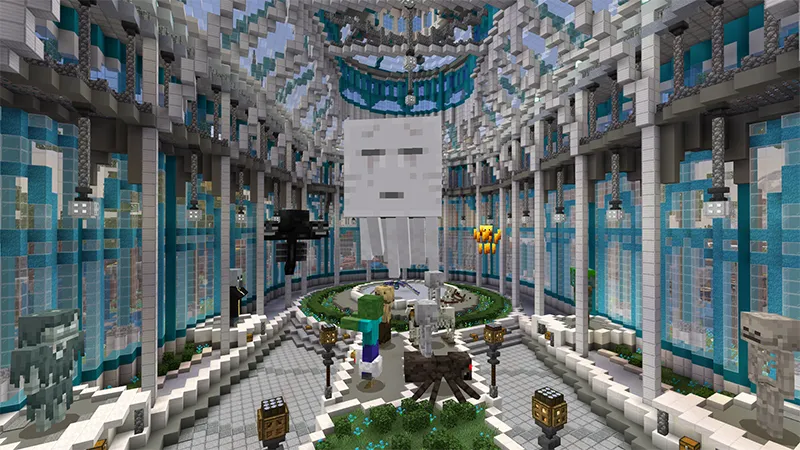
\includegraphics[width=\linewidth]{figures/minecraft_complexity.png}
    \caption{A player-built structure from the 10th Anniversary Celebration map, illustrating the spatial and visual complexity characteristic of Minecraft environments. Answering questions about structures, biomes, or mechanics often requires images alongside text.}
    \label{fig:minecraft_complexity}
\end{figure}

\begin{figure}[htbp]
    \centering
    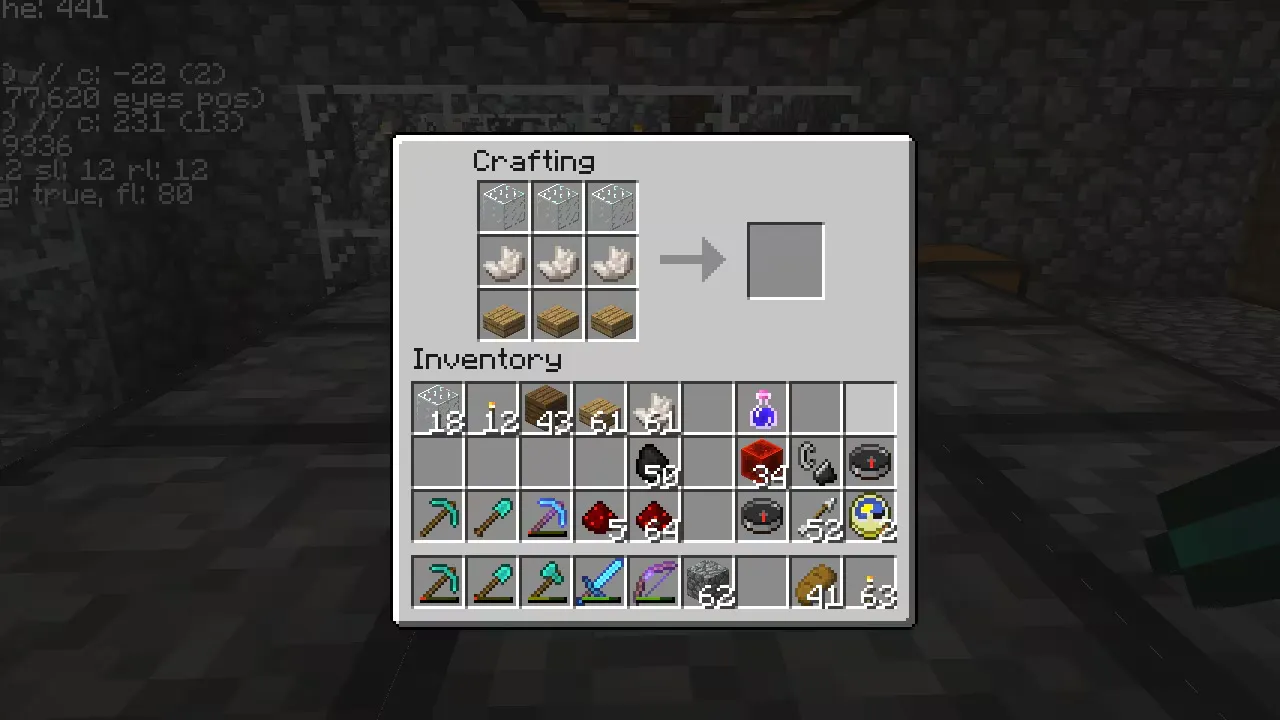
\includegraphics[width=\linewidth]{figures/crafting_recipe_book.png}
    \caption{A crafting recipe grid (e.g., Daylight Detector), showing the precise ingredient requirements needed to construct items. A 1-cell shift or incorrect material variant produces an entirely different item or fails silently; this scale of structured visual-spatial knowledge is ill-suited to parametric LLM recall.}
    \label{fig:crafting_recipe_book}
\end{figure}

\begin{itemize}
    \item \textbf{Visual-spatial reasoning}: Many answers are incomprehensible without image context (e.g., redstone circuit diagrams, biome terrain features, mob spawn conditions).
    \item \textbf{Recipe breadth}: Hundreds of crafting recipes with exact positional constraints; a 1-cell shift produces an entirely different item or fails silently.
    \item \textbf{Version fragmentation}: Mechanics, item IDs, and behaviors differ substantially between Java Edition, Bedrock Edition, and legacy console releases. A query without version context is genuinely ambiguous.
    \item \textbf{Encyclopedic depth}: The wiki spans 12,487 articles covering biomes, entities, blocks, items, structures, mechanics, commands, and changelogs, far exceeding the context window of any single LLM call.
\end{itemize}

\subsection{Query Complexity and Scale}

The 333-pair evaluation set spans three difficulty tiers. Easy questions target single-fact lookups; medium questions require synthesising information across infoboxes or related sections; hard questions demand cross-mechanic or cross-edition reasoning. This last category is where purely parametric LLMs fail most often, because the answer typically depends on exact numeric or version-conditional details scattered across multiple wiki sections.

\subsection{Failure Modes of Existing Solutions}

General-purpose LLMs fail in this domain by confabulating specifics, flattening visual structure, and missing post-pretraining game changes. Ore-acle addresses these failure modes by grounding generation in retrieved chunks, preserving structured wiki content during preprocessing, and attaching precise inline citations and images to each response.

\section{System Architecture}

\subsection{Offline Pipeline}

Ore-acle ingests 12,487 HTML pages from the Minecraft Wiki, producing 94,404 section-aware chunks, 78,172 LangChain comparison chunks, and 61,248 locally stored images. Figure~\ref{fig:data_pipeline} summarizes the end-to-end offline pipeline. The key design choice is that preprocessing is not treated as a generic cleaning stage: it is where much of the downstream retrieval quality is won or lost.

Two pipeline decisions are especially important. First, the text cleaner preserves infoboxes and extracts Minecraft UI recipe widgets directly from CSS grids into text-searchable representations such as \texttt{[Crafting Recipe: [., ., .] [Diamond, Book, Diamond] ...]}. This allows both dense and sparse retrievers to index crafting layouts that would otherwise remain buried in presentational HTML. Second, the chunker is explicitly wiki-aware: it preserves list blocks, splits text at sentence boundaries, removes pure navigation sections, and merges sub-threshold orphan chunks backward into the previous content chunk when this stays within budget. These heuristics reduce ranking noise and keep technical details attached to the local context that makes them interpretable.

For all main experiments, we use \texttt{nomic-ai/nomic-embed-text-v1.5}~\cite{nomic2024} as the default dense encoder because it wins the embedding ablation on both text retrieval and image recall. BAAI/bge-m3~\cite{bge2024} and multilingual-E5-Large~\cite{wang2022text} are evaluated separately in Section~\ref{sec:embedding-axis}.

\begin{figure*}[ht]
\centering
\resizebox{\textwidth}{!}{%
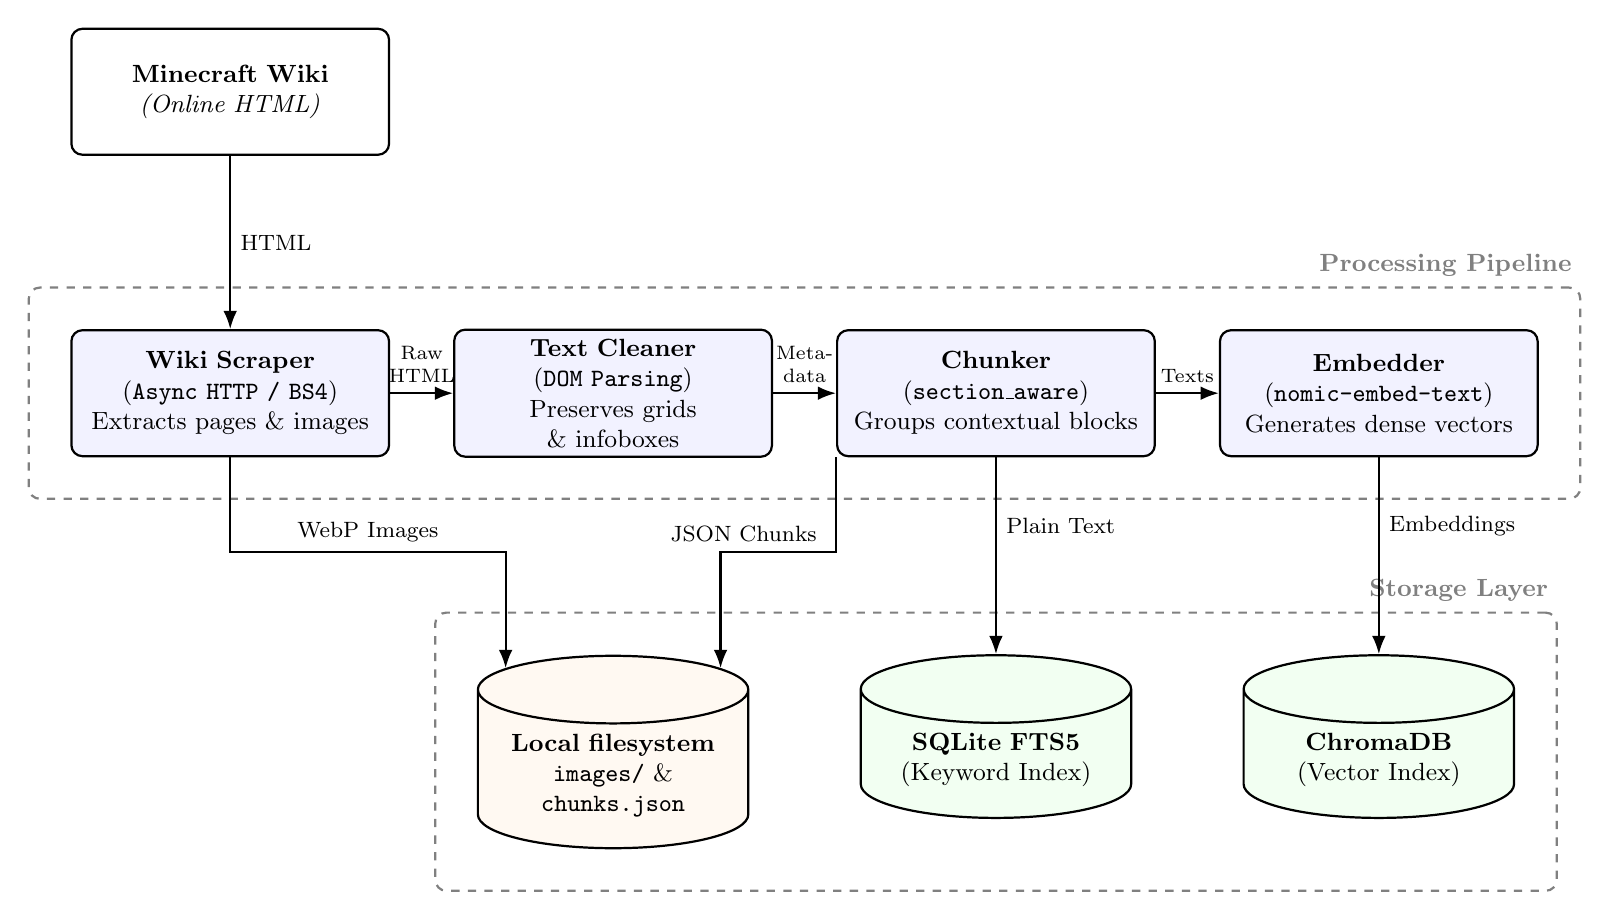
\begin{tikzpicture}[
    node distance=1.5cm and 0.8cm,
    box/.style={rectangle, draw=black, thick, fill=blue!5, text width=3.8cm, align=center, rounded corners, minimum height=1.6cm, font=\small},
    dbbox/.style={cylinder, draw=black, thick, fill=green!5, shape border rotate=90, aspect=0.25, text width=3.2cm, align=center, minimum height=1.8cm, font=\small},
    arrow/.style={-Latex, thick},
    group/.style={rectangle, draw=gray, dashed, thick, rounded corners, inner sep=15pt}
]
    % Processing Pipeline Row
    \node[box] (scraper) {\textbf{Wiki Scraper}\\(\texttt{Async HTTP / BS4})\\Extracts pages \& images};
    \node[box, right=of scraper] (cleaner) {\textbf{Text Cleaner}\\(\texttt{DOM Parsing})\\Preserves grids \& infoboxes};
    \node[box, right=of cleaner] (chunker) {\textbf{Chunker}\\(\texttt{section\_aware})\\Groups contextual blocks};
    \node[box, right=of chunker] (embedder) {\textbf{Embedder}\\(\texttt{nomic-embed-text})\\Generates dense vectors};
    
    % Grouping boxes (Define pipeline group early to use for wiki placement)
    \node[group, fit=(scraper) (embedder)] (pipeline) {};
    \node[anchor=south east, font=\bfseries\small, color=gray] at (pipeline.north east) {Processing Pipeline};

    % Data Source (Above Scraper, but higher to avoid label overlap)
    \node[box, fill=white, above=2.2cm of scraper] (wiki) {\textbf{Minecraft Wiki}\\\textit{(Online HTML)}};

    % Storage Layer Row (increased distance to 3cm to allow clean arrow routing between groups)
    \node[dbbox, fill=orange!5, below=2.5cm of cleaner] (localfs) {\textbf{Local filesystem}\\ \texttt{images/} \& \texttt{chunks.json}};
    \node[dbbox, below=2.5cm of chunker] (sqlite) {\textbf{SQLite FTS5}\\(Keyword Index)};
    \node[dbbox, below=2.5cm of embedder] (chroma) {\textbf{ChromaDB}\\(Vector Index)};
    
    \node[group, fit=(localfs) (chroma)] (storage) {};
    \node[anchor=south east, font=\bfseries\small, color=gray] at (storage.north east) {Storage Layer};

    % Arrows Main Flow
    \draw[arrow] (wiki) -- node[right]{\footnotesize HTML} (scraper);
    \draw[arrow] (scraper) -- node[above, align=center]{\scriptsize Raw \\[-0.8ex] \scriptsize HTML} (cleaner);
    \draw[arrow] (cleaner) -- node[above, align=center]{\scriptsize Meta- \\[-0.8ex] \scriptsize data} (chunker);
    \draw[arrow] (chunker) -- node[above]{\scriptsize Texts} (embedder);
    
    % Arrows to Storage (Routed precisely in the middle of the 2.5cm gap)
    \draw[arrow] (scraper.south) -- ++(0,-1.2) -| node[pos=0.25, above]{\footnotesize WebP Images} (localfs.north west);
    \draw[arrow] (chunker.south west) -- ++(0,-1.2) -| node[pos=0.4, above]{\footnotesize JSON Chunks} (localfs.north east);
    \draw[arrow] (chunker.south) -- node[pos=0.35, right]{\footnotesize Plain Text} (sqlite.north);
    \draw[arrow] (embedder.south) -- node[pos=0.35, right]{\footnotesize Embeddings} (chroma.north);
    
\end{tikzpicture}%
}
\caption{Ore-acle Offline Data Pipeline: From live Minecraft Wiki to hybrid local storage.}
\label{fig:data_pipeline}
\end{figure*}

\subsection{Retrieval Architecture}

\textbf{Storage Strategy:} ChromaDB stores dense embeddings for the section-aware and LangChain chunk collections; SQLite FTS5 stores the full keyword index over section-aware chunks; and the local filesystem stores WebP images referenced by hash-based filenames.

\textbf{Runtime Query Flow:}
\begin{figure}[htbp]
    \centering
    \definecolor{moeorange}{RGB}{252,223,189}
    \definecolor{attnblue}{RGB}{196,213,242}
    \definecolor{basegray}{RGB}{240,240,240}
    \definecolor{arrowred}{RGB}{135,63,73}
    \begin{tikzpicture}[
        scale=0.7, transform shape,
        node distance=0.8cm and 0.5cm,
        basebox/.style={rectangle, draw=black, thick, text centered, rounded corners=3pt, minimum height=0.7cm, minimum width=4cm, inner sep=5pt},
        bluebox/.style={basebox, fill=attnblue},
        orangebox/.style={basebox, fill=moeorange},
        graybox/.style={basebox, fill=basegray},
        plainbox/.style={basebox, fill=white},
        arrow/.style={thick,->,>=stealth, draw=black},
        redarrow/.style={thick,->,>=stealth, draw=arrowred},
        ]
        
        \node (user) [plainbox] {User Query};
        \node (api) [graybox, below=of user] {FastAPI Server};
        \node (hybrid) [bluebox, below=1.2cm of api] {Hybrid Search Module};
        
        \node (chroma) [orangebox, below left=of hybrid, xshift=1.5cm, yshift=-0.5cm] {ChromaDB (Semantic)};
        \node (sqlite) [orangebox, below right=of hybrid, xshift=-1.5cm, yshift=-0.5cm] {SQLite FTS5 (Keyword)};
        
        \node (plus) [circle, draw=black, thick, inner sep=2pt, below=2cm of hybrid] {$\oplus$};
        
        \node (rrf) [bluebox, below=0.5cm of plus] {Reciprocal Rank Fusion};
        \node (reranker) [graybox, draw=black!60, dashed, below=0.5cm of rrf] {Reranker (optional)};
        \node (topk) [graybox, below=1.2cm of reranker] {Top-K Retrieval ($K=5/10$)};
        \node (llm) [orangebox, below=of topk] {LLM Generation};
        \node (response) [plainbox, below=of llm] {Response + Citations};
        
        \draw [arrow] (user) -- (api);
        \draw [arrow] (api) -- (hybrid);
        \draw [arrow] (hybrid) -| (chroma);
        \draw [arrow] (hybrid) -| (sqlite);
        \draw [redarrow] (chroma) |- (plus);
        \draw [redarrow] (sqlite) |- (plus);
        \draw [redarrow] (plus) -- (rrf);
        \draw [arrow] (rrf) -- (reranker);
        \draw [arrow] (reranker) -- (topk);
        \draw [arrow] (topk) -- (llm);
        \draw [arrow] (llm) -- (response);
        
        % Background dashed box
        \node[rectangle, draw=black, dashed, thick, rounded corners=5pt, fit=(hybrid) (chroma) (sqlite) (rrf) (reranker), inner sep=10pt, yshift=2pt] (group) {};
        
    \end{tikzpicture}
    \caption{Runtime hybrid search pipeline with optional cross-encoder reranker applied post-RRF fusion.}
    \label{fig:query_flow}
\end{figure}

The dense retriever alone is strong, but Ore-acle's main systems contribution is making sparse retrieval competitive enough to help rather than harm fusion. Out-of-the-box FTS5 fails on natural-language technical questions because player-phrased queries rarely match wiki text verbatim: the query ``how do I breed pigs'' would require a wiki sentence containing all four words, which does not exist. We therefore rewrite queries into OR-connected term sets, remove hardcoded stopwords, and apply title-weighted BM25 scoring so exact article-title matches receive much higher priority than body-only matches. This tuned keyword channel raises the sparse baseline from MRR 0.425 to 0.515 and is what makes weighted RRF useful rather than cosmetic.

Ore-acle uses chunk-level provenance rather than page-level citations. Each retrieved chunk carries page title, section heading, page URL, and the exact text span shown to the model. The final answer cites these chunks inline with \texttt{[n]} markers, allowing a reader to inspect a specific supporting section instead of an entire wiki page. This design choice is central to the high citation-faithfulness scores reported later, and it makes factual inspection practical for technical wiki questions.

\subsection{Generation with Citations}

Responses use NotebookLM-style inline citations with verbatim grounding, explicit page titles, and original URLs. When relevant images are available, the system injects them alongside the answer so that recipe layouts, structures, and other visual mechanics are not reduced to plaintext alone.

\subsection{UI Walkthrough \& Multimodal Capabilities}
The frontend is a lightweight chat interface whose main research role is to demonstrate grounded output rather than novel interaction design. Users may provide screenshots as additional multimodal context, which are appended to the prompt alongside retrieved wiki chunks. Figure~\ref{fig:ui_crafting} illustrates the resulting behavior: the system answers a gameplay question with inline citations and an explicitly rendered crafting layout instead of forcing the model to paraphrase a recipe from memory.

\begin{figure}[htbp]
    \centering
    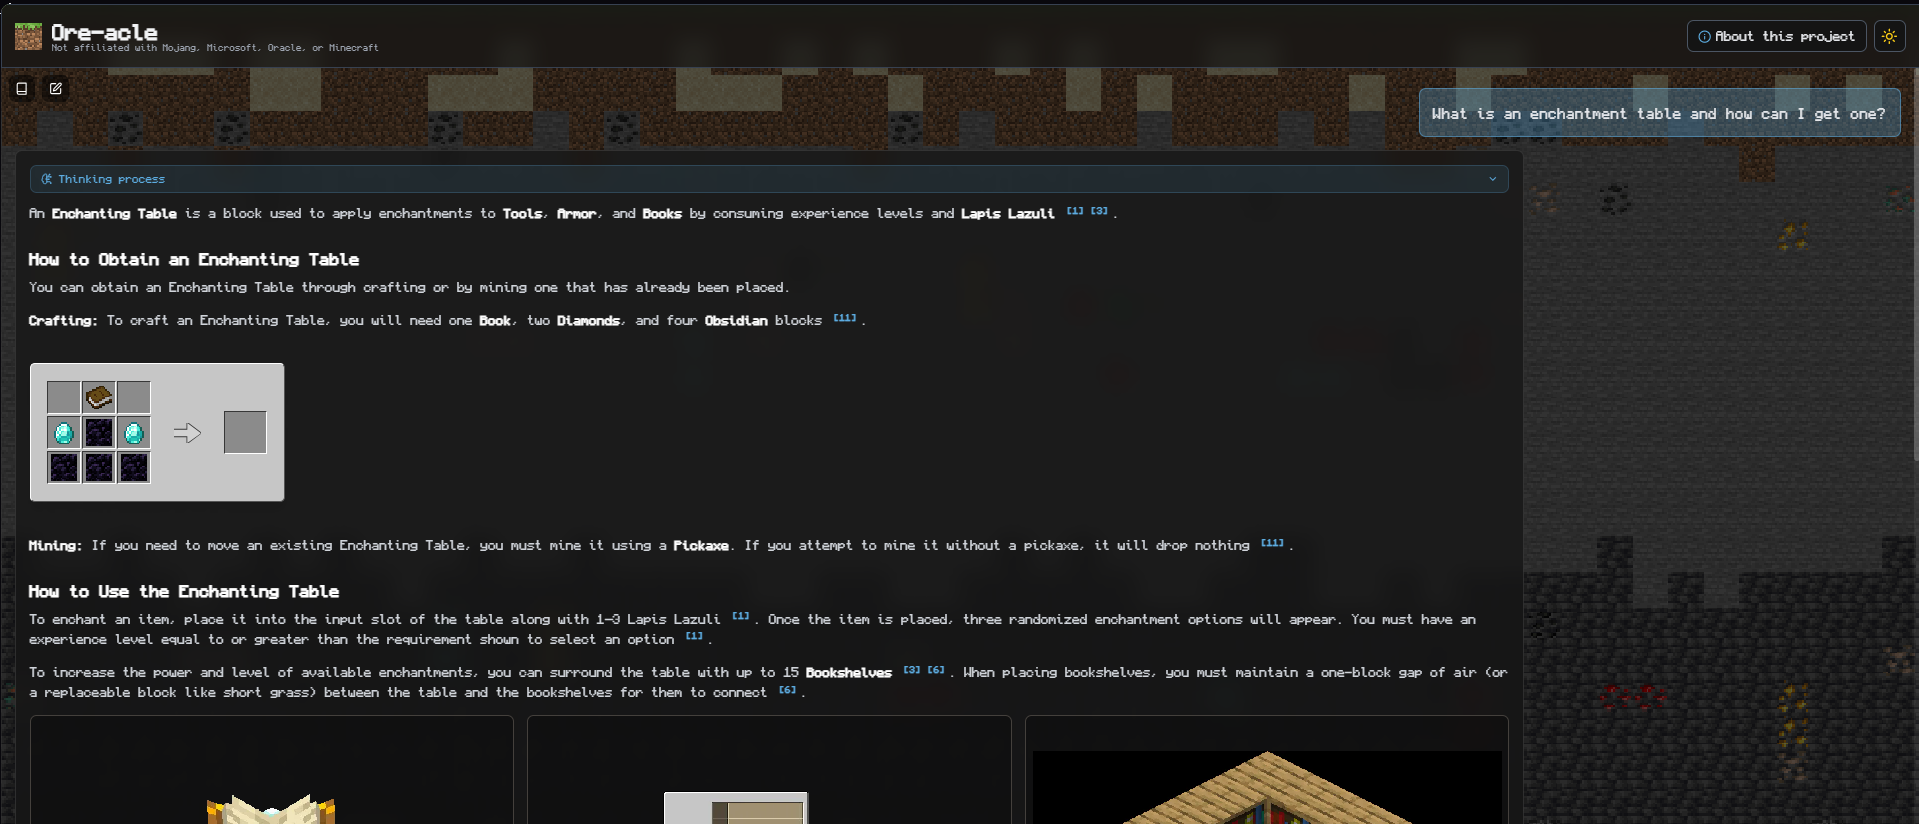
\includegraphics[width=\linewidth]{figures/UI_show_crafting.png}
    \caption{Ore-acle UI response to the query ``What is an enchantment table and how can I get one?'' The system retrieves the relevant wiki chunks and renders the crafting recipe grid (Book, two Diamonds, four Obsidian) inline within the response, alongside inline citations. This demonstrates the system's multimodal grounding: structured recipe data extracted from wiki CSS grids is presented visually rather than as raw text.}
    \label{fig:ui_crafting}
\end{figure}

\section{Experimental Setup}

\subsection{Dataset}

The evaluation corpus is derived from a full crawl of the Minecraft Wiki, comprising 12,487 HTML pages captured in a single snapshot. Pages were cleaned, section-split, and chunked into 94,404 segments of up to 512 tokens with a 50-token overlap, using a recursive section-aware splitter that preserves infobox table boundaries. Concurrently, 61,248 images were downloaded, decoded to WebP, and stored under content-addressed filenames derived from their source URLs.

The golden test set consists of 333 question-answer pairs generated via Gemini Flash Lite~\cite{gemini2023}. One hundred twenty source pages were selected using a PageRank-plus-content-density heuristic so that the benchmark emphasizes high-value, well-linked wiki pages rather than uniformly random articles. For each page, three questions were generated at easy, medium, and hard difficulty, then manually reviewed. Additional adversarial prompts were seeded to probe ambiguous or narrative questions outside straightforward mechanics lookups.

\subsection{Evaluation Framework}

\footnote{Evaluations tracking latency were conducted on consumer hardware (Intel Core i5-12450H, 16\,GB DDR4, NVIDIA RTX 4060 8\,GB VRAM) entirely locally to validate baseline accessibility.}

\textbf{Golden Test Set Generation:}
\begin{itemize}
    \item 333 question-answer pairs spanning explicit game mechanics, lore, and structural challenges.
    \item Generated via Gemini Flash Lite (OpenRouter) with a two-pass image verification protocol.
    \item Inclusion of manually seeded adversarial/narrative edge cases (e.g., "Who is Steve?", "Best gearsets") to secure generation robustness against trivia blindspots.
    \item Streaming JSON processing via \texttt{ijson} applied for localized memory parsing efficiency.
\end{itemize}

\textbf{Two-Phase Ablation Protocol:}

\begin{table}[h]
\caption{Ablation study design}
\label{tab:ablation}
\centering
\begin{tabular}{lll}
\toprule
\textbf{Phase} & \textbf{Axis} & \textbf{Configurations} \\
\midrule
1: Retriever & Search Mode & Semantic / Keyword / Hybrid \\
 & Embedding & BAAI/bge-m3 / Nomic / E5-Large \\
 & Chunking & Section-aware / LangChain \\
 & Reranker & No reranker / BGE v2-m3 / Qwen3-0.6B / Qwen3-4B / zerank-2 \\
\midrule
2: Generator & LLM & Gemma 4 e2B / e4B / 31B / Gemini Flash Lite \\
\bottomrule
\end{tabular}

\end{table}

\subsection{Metrics}

\begin{table}[h]
\caption{Evaluation metrics}
\label{tab:metrics}
\centering
\begin{tabular}{lp{8cm}}
\toprule
\textbf{Metric} & \textbf{Description} \\
\midrule
Recall@5/10 & Proportion of relevant chunks in top-K \\
Precision@10 & Accuracy of top-10 retrieved chunks \\
MRR & Mean Reciprocal Rank of first relevant result \\
Image Recall & Proportion of questions with correct image retrieval \\
Token F1 & Lexical overlap between generated and gold answer \\
ROUGE-L & Longest common subsequence for answer quality \\
\bottomrule
\end{tabular}

\end{table}

\subsection{Baselines}

All retrieval configurations are evaluated relative to a semantic-only dense retriever using \texttt{nomic-embed-text-v1.5}. Keyword-only search provides a sparse lower bound, and the hybrid RRF configuration sweeps $\alpha \in \{0.0, 0.2, \ldots, 1.0\}$ to quantify how much sparse evidence should influence the final ranking.



\section{Results and Ablation Studies}

\subsection{Search Mode Ablation}

\textbf{Configuration:} 333-pair questionset, nomic-embed-text-v1.5 embeddings, section-aware chunking

\begin{table}[h]
\caption{Search mode comparison. Best scores in bold.}
\label{tab:search-mode}
\centering
\begin{tabular}{lcccc}
\toprule
\textbf{Mode} & \textbf{MRR} & \textbf{R@5} & \textbf{R@10} & \textbf{Img Rcl} \\
\midrule
\textbf{Semantic} & \textbf{0.625} & \textbf{0.458} & \textbf{0.514} & \textbf{0.290} \\
Keyword (OOTB, length-filter) & 0.425 & 0.358 & 0.465 & 0.102 \\
Keyword (Custom BM25) & 0.515 & 0.407 & 0.490 & 0.131 \\
Hybrid (RRF, $\alpha$=0.80) & 0.612 & 0.449 & 0.516 & 0.265 \\
\bottomrule
\end{tabular}

\end{table}

\textbf{Key Finding:} The main result of Table~\ref{tab:search-mode} is not simply that semantic retrieval is strong; it is that sparse retrieval only becomes competitive after domain-specific tuning. Replacing default FTS5 behavior with OR semantics, stopword filtering, stemming, and heavy title weighting raises keyword MRR from 0.425 to 0.515, a 21\% relative gain. Pure semantic retrieval still achieves the best MRR (0.625), but hybrid search remains the operational choice because it preserves near-peak text quality while maintaining stronger multimodal grounding than either sparse baseline.

\begin{figure}[h]
\centering
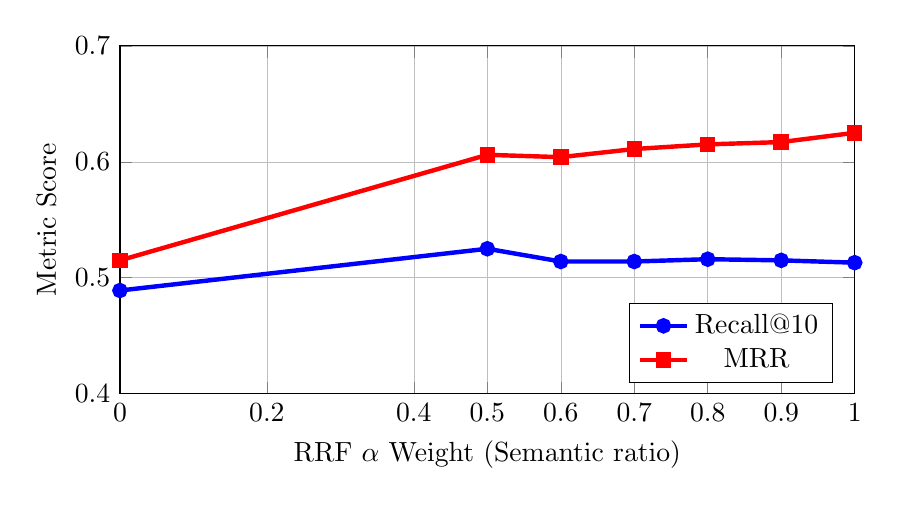
\begin{tikzpicture}
\begin{axis}[
    width=0.9\linewidth,
    height=6cm,
    xlabel={RRF $\alpha$ Weight (Semantic ratio)},
    ylabel={Metric Score},
    xmin=0, xmax=1,
    ymin=0.4, ymax=0.7,
    xtick={0, 0.2, 0.4, 0.5, 0.6, 0.7, 0.8, 0.9, 1.0},
    legend pos=south east,
    grid=both,
    grid style={line width=.1pt, draw=gray!20},
    major grid style={line width=.2pt,draw=gray!50},
    every axis plot/.append style={ultra thick}
]

\addplot[color=blue, mark=*] coordinates {
    (0.00, 0.489) % Keyword
    (0.50, 0.525)
    (0.60, 0.514)
    (0.70, 0.514)
    (0.80, 0.516)
    (0.90, 0.515)
    (1.00, 0.513) % Semantic
};
\addlegendentry{Recall@10}

\addplot[color=red, mark=square*] coordinates {
    (0.00, 0.515) % Keyword
    (0.50, 0.606)
    (0.60, 0.604)
    (0.70, 0.611)
    (0.80, 0.615)
    (0.90, 0.617)
    (1.00, 0.625) % Semantic
};
\addlegendentry{MRR}

\end{axis}
\end{tikzpicture}
\caption{Effect of RRF $\alpha$ parameter on Retrieval Quality (333-question set). $\alpha=0$ represents pure keyword, while $\alpha=1$ is pure semantic search. $\alpha=0.80$ achieves the best Recall@10 among hybrid configurations while maintaining near-peak MRR.}
\label{fig:alpha_sweep}
\end{figure}

The $\alpha$ sweep shows that the dense retriever should dominate fusion, but not entirely. Moving from $\alpha=0$ to $\alpha=0.80$ yields a steep gain in MRR, after which returns diminish; the remaining keyword contribution is still useful for article-title matches and exact lexical cues that help multimodal retrieval. This explains why Ore-acle locks $\alpha$=0.80 (80\% semantic weight, 20\% keyword) rather than defaulting to pure semantic search in deployment.

\subsection{Embedding Model Ablation}
\label{sec:embedding-axis}

\textbf{Configuration:} 333-pair questionset, section-aware chunking, hybrid search ($\alpha$=0.80, $K$=20)

\begin{table}[h]
\caption{Embedding model comparison. Best scores in bold.}
\label{tab:embedding}
\centering
\begin{tabular}{llcccc}
\toprule
\textbf{Model} & \textbf{Dim} & \textbf{MRR} & \textbf{R@5} & \textbf{R@10} & \textbf{Img Rcl} \\
\midrule
\texttt{nomic-embed-text-v1.5} & 768 & \textbf{0.612} & \textbf{0.455} & \textbf{0.519} & \textbf{0.265} \\
\texttt{BAAI/bge-m3} & 1024 & 0.605 & 0.454 & 0.512 & 0.225 \\
\texttt{multilingual-e5-large} & 1024 & 0.508 & 0.371 & 0.432 & 0.141 \\
\bottomrule
\end{tabular}

\end{table}

\textbf{Key Findings:} \texttt{nomic-embed-text-v1.5} wins on every reported retrieval metric, so it remains the default model for all subsequent ablations. \texttt{bge-m3} is close on text metrics but weaker on image recall; \texttt{multilingual-e5-large} trails substantially, suggesting that its multilingual objective is not the right fit for this English-only technical corpus.


\subsection{Chunking Strategy Ablation}
\label{sec:chunking-axis}

Preserving semantic boundaries is especially important in wiki corpora, where a short subsection often only makes sense in the context of the section directly above it. Our section-aware chunker therefore does more than respect headings: it preserves list blocks as atomic units, performs sentence-boundary overlap for prose, skips pure navigation sections that pollute ranking, and merges sub-threshold chunks back into the previous content chunk when possible. This absorb-backward rule is designed for common wiki artifacts such as short trailing subsections, ``See also'' stubs, and fragmented mechanic notes. We compare this strategy against LangChain \texttt{RecursiveCharacterTextSplitter} under the same embedding and hybrid-retrieval configuration.

\begin{table}[h]
\caption{Chunking strategy comparison (nomic-ai/nomic-embed-text-v1.5, hybrid $\alpha$=0.80). Best scores in bold.}
\label{tab:chunking}

\centering
\begin{tabular}{lccccc}
\toprule
\textbf{Strategy} & \textbf{MRR} & \textbf{R@5} & \textbf{R@10} & \textbf{Img Rcl} \\
\midrule
\textbf{Section-Aware} & \textbf{0.636} & \textbf{0.488} & \textbf{0.572} & \textbf{0.279} \\
LangChain$^\dagger$ & 0.614 & 0.462 & 0.517 & 0.203 \\
\bottomrule
\end{tabular}
\end{table}

\textbf{Key Finding:} The custom section-aware chunking strategy effectively retains wiki article structure, generating semantically coherent chunks that achieve comparable text retrieval to LangChain while providing superior image grounding. Section-aware chunking is the definitive choice for wiki RAG. We note that this comparison is holistic; isolating the contribution of individual heuristics (navigation filtering, absorb-backward merging, list preservation) remains future work.

\subsection{Reranker Ablation}
\label{sec:reranker-axis}

\textbf{Configuration:} 333-pair questionset, nomic-embed-text-v1.5, section-aware chunking, hybrid search ($\alpha$=0.80). All rerankers are applied post-RRF over a widened candidate pool of 30 chunks, re-ranking to the final top-10. Latency is reported per query on consumer hardware (RTX~4060 8\,GB VRAM, Intel Core i5-12450H).

\begin{table}[h]
\caption{Reranker comparison (hybrid, nomic-embed-text-v1.5, section-aware, 333 questions). PassR@10 = passage-level span recall at 10. Best scores in bold.}
\label{tab:reranker}
\centering
\begin{tabular}{lcccccc}
\toprule
\textbf{Reranker} & \textbf{MRR} & \textbf{R@5} & \textbf{R@10} & \textbf{Img Rcl} & \textbf{PassR@10} & \textbf{Latency} \\
\midrule
No reranker         & 0.612 & 0.452 & 0.518 & 0.265 & 0.508 & 0.2\,s \\
BGE Reranker v2-m3  & 0.604 & 0.456 & 0.520 & 0.230 & 0.535 & 3.7\,s \\
Qwen3-Reranker-0.6B & 0.604 & 0.448 & 0.526 & \textbf{0.317} & 0.542 & 2.0\,s \\
Qwen3-Reranker-4B   & \textbf{0.636} & 0.472 & 0.543 & \textbf{0.317} & \textbf{0.568} & 33.0\,s \\
\textbf{zerank-2}   & \textbf{0.636} & \textbf{0.483} & \textbf{0.571} & 0.203 & 0.547 & 13.3\,s \\
\bottomrule
\end{tabular}
\end{table}

\textbf{Key Findings:} Reranking improves retrieval quality materially only when the reranker is sufficiently capable. BGE Reranker v2-m3 \textit{decreases} MRR from 0.612 to 0.604 and image recall from 0.265 to 0.230, suggesting its scoring function does not align well with Minecraft-specific technical query semantics. Qwen3-Reranker-0.6B recovers recall (R@10=0.526) at only 2.0\,s latency and uniquely achieves the highest image recall (0.317), making it an attractive lightweight option when multimodal grounding is the priority. Qwen3-Reranker-4B and zerank-2 tie on MRR (0.636), but zerank-2 substantially outperforms on Recall@10 (0.571 vs.\ 0.543) at less than half the latency (13.3\,s vs.\ 33.0\,s). zerank-2 is therefore the recommended post-retrieval component for deployments where text retrieval quality and interactive latency both matter.

\subsection{Generator Evaluation}

\textbf{Configuration:} 333-pair questionset, nomic-embed-text-v1.5 embeddings, section-aware chunking, hybrid search ($\alpha$=0.80). All models were prompted with identical system instructions requiring inline \texttt{[n]} citations. We evaluate four models: Gemma 4 e2B, Gemma 4 e4B, and Gemma 4 31B~\cite{gemma2024}, alongside Gemini Flash Lite~\cite{gemini2023}. We purposefully select this spread to evaluate whether highly-grounded retrieved context allows ultra-small, edge-deployable models (e2B/e4B parameters) to punch above their weight against state-of-the-art frontier models.

\begin{table}[h]
\caption{Generator evaluation (333-question set). CitF = Citation Faithfulness. Latency excluded: Ollama (local) and OpenRouter (API) are not comparable on this axis. Best scores in bold.}
\label{tab:generator}
\centering
\begin{tabular}{llcccc}
\toprule
\textbf{Model} & \textbf{Backend} & \textbf{Avg F1} & \textbf{ROUGE-L} & \textbf{BERTScore} & \textbf{CitF} \\
\midrule
Gemma 4 e2B & Ollama (local)      & 0.244 & 0.163 & 0.711 & 0.634 \\
Gemma 4 e4B & Ollama (local)      & 0.108 & 0.074 & 0.310 & 0.295 \\
\textbf{Gemma 4 31B}   & OpenRouter (API)    & \textbf{0.290} & \textbf{0.174} & 0.844 & 0.973 \\
Gemini Flash Lite & OpenRouter (API) & 0.288 & 0.168 & \textbf{0.844} & \textbf{0.983} \\
\bottomrule
\end{tabular}

\end{table}

\textbf{Key Finding:} Once retrieval is well tuned, generator choice matters less than expected for factual grounding. The strongest cloud models tie on BERTScore and achieve near-perfect citation faithfulness, while Gemma 4 e2B remains surprisingly viable given its size. Gemma 4 e4B's low average (F1=0.108) reflects a high rate of empty responses rather than uniformly poor quality; when it does answer, its responses are factually grounded (F1 0.32--0.60). This likely stems from finetuning brittleness with the strict inline-citation format. Overall, retrieval and provenance design, rather than sheer generator scale, are the primary determinants of answer reliability in this setting.

\subsection{Qualitative Examples}
\label{sec:qualitative}

We keep two representative examples in the main paper: one factual lookup that benefits from structured grounding, and one hard cross-edition query that tests whether the system can preserve subtle mechanic distinctions.

\subsubsection*{Easy: Factual Drop Query}

\textbf{Query:} \textit{``What does a Blaze drop?''}

Ore-acle retrieves nine chunks from the \textit{Blaze} and \textit{Blaze Powder} wiki pages and produces a structured response with inline citations and a programmatically generated Looting table:

\begin{lstlisting}
When killed by a player or a tamed wolf, a Blaze drops:

- Blaze Rod [1][4]: drop rate increases with Looting.
  | Looting Level | Expected Drops |
  | None          | 0.50           |
  | Looting I     | 0.75           |
  | Looting II    | 1.00           |
  | Looting III   | 1.25           |

- Experience Orbs: 10 XP per kill [1].

Blaze Rods are a primary ingredient for Blaze Powder,
required to fuel Brewing Stands and craft Eyes of Ender [6].
The "Into Fire" advancement is associated with their
acquisition [7][9].
\end{lstlisting}

\noindent The model correctly produces version-specific historical trivia (Legacy Console glowstone dust drops) attributed to the correct source chunk, demonstrating that fine-grained infobox knowledge is retrieved and cited rather than hallucinated.

\subsubsection*{Hard: Cross-Edition Mechanic Reasoning}

\textbf{Query:} \textit{``How does the Bad Omen effect change raid scaling?''}

This question requires reconciling Java and Bedrock Edition semantics, a class of query where parametric LLMs frequently confabulate. Ore-acle retrieves ten chunks spanning the \textit{Bad Omen}, \textit{Ominous Bottle}, \textit{Raid}, and \textit{Illager} pages, and explicitly partitions its answer by edition:

\begin{lstlisting}
Java Edition:
- Higher Bad Omen levels increase raider enchantment
  probability [1][2][4][9].
- Bad Omen II or higher triggers an additional raid wave [1][4].
- Hero of the Village effect level matches the triggering
  Bad Omen level [1][10].

Bedrock Edition:
- Bad Omen level has no effect on raid scaling [1].

Note: Bad Omen affects Trial Spawners (converting them to
Ominous Trial Spawners), but the level does not change trial
difficulty [1][4].
\end{lstlisting}

\noindent The Java/Bedrock asymmetry (higher Bad Omen is meaningless on Bedrock) is precisely the kind of technical distinction that general LLMs often conflate. Ore-acle correctly surfaces the \texttt{Bad Omen/Before 1.21} chunk to capture the historical context of the mechanic's redesign in Java Edition 1.21.

\section{Discussion}

\subsection{Keyword Parameter Tuning within Technical Domains}

The SQLite FTS5 index uses OR-connected query semantics rather than exact-match, a configuration choice with significant recall impact. Under naive exact-match semantics, multi-word natural language queries return near-zero results because the wiki corpus does not contain verbatim question phrasing. Switching to OR semantics, while filtering single-character tokens as stopwords, raised keyword Recall@10 from effectively 0 to 0.490 (Table~\ref{tab:search-mode}), enabling meaningful comparison with the dense retriever. This highlights that keyword retrieval in structured technical corpora requires query-side adaptation: the precision/recall tradeoff is not symmetric with general-domain BM25 assumptions.

\subsection{Design Implications for Wiki RAG}
\textbf{Winning Configuration:} Hybrid search ($\alpha$=0.80, nomic-embed-text-v1.5, section-aware chunking) with zerank-2 reranker. This configuration achieves MRR=0.636, R@10=0.571, and Image Recall=0.203

Four design lessons emerge from the ablations. First, domain-specific preprocessing matters: navigation filtering, chunk merging, and recipe-grid extraction materially improve what the retriever can index. Second, sparse retrieval should not be treated as an untuned baseline; in structured technical corpora, query semantics and field weighting determine whether keyword search is useful at all. Third, reranker selection is non-trivial: a standard cross-encoder (BGE Reranker v2-m3) \textit{hurts} MRR in this domain, while only sufficiently capable models (Qwen3-4B, zerank-2) deliver meaningful gains over the unranked baseline. Fourth, image recall and text retrieval trade off across configurations---the reranker that maximises Recall@10 (zerank-2) is not the one that maximises image recall (Qwen3-Reranker-0.6B) so the operational choice depends on the application's modality requirements.

\begin{thebibliography}{99}

\bibitem[Cormack et al.(2009)]{cormack2009reciprocal}
G.~V.~Cormack, C.~L.~A.~Clarke, and S.~Buettcher.
\newblock Reciprocal Rank Fusion outperforms Condorcet and individual rank learning methods.
\newblock \textit{SIGIR '09}, pages 758--759, 2009.

\bibitem[Gao et al.(2023)]{gao2023retrieval}
Y.~Gao, Y.~Xiong, X.~Gao, K.~Jia, J.~Pan, Y.~Bi, Y.~Dai, J.~Sun, and H.~Wang.
\newblock Retrieval-Augmented Generation for Large Language Models: A Survey.
\newblock \textit{arXiv:2312.10997}, 2023.

\bibitem[Google(2023)]{notebooklm2023}
Google.
\newblock NotebookLM: AI Research Tool with verifiable inline citations, 2023.
\newblock \url{https://notebooklm.google}

\bibitem[Kshirsagar(2024)]{kshirsagar2024enhancing}
A.~Kshirsagar.
\newblock Enhancing RAG Performance Through Chunking and Text Splitting Techniques.
\newblock \textit{Int. J. Sci. Res. Comput. Sci. Eng. Inf. Technol.}, 10:151--158, 2024.

\bibitem[Kumar(2025)]{kumar2025wikipedia}
R.~Kumar.
\newblock Wikipedia-Savvy-RAG: A Lightweight Retrieval-Augmented Generation System for STEM Question.
\newblock In \textit{Proc. Int. Conf. Recent Advancements in Artificial Intelligence}, 2025.

\bibitem[Li et al.(2025)]{li2025enhancing}
S.~Li, L.~Stenzel, C.~Eickhoff, and S.~A. Bahrainian.
\newblock Enhancing Retrieval-Augmented Generation: A Study of Best Practices.
\newblock \textit{arXiv:2501.07391}, 2025.

\bibitem[Yu et al.(2024)]{yu2024evaluation}
H.~Yu et~al.
\newblock Evaluation of Retrieval-Augmented Generation: A Survey.
\newblock \textit{arXiv:2405.07437}, 2024.

\bibitem[Chen et al.(2024)]{bge2024}
J.~Chen et~al.
\newblock BGE M3-Embedding: Multi-Lingual, Multi-Functionality, Multi-Granularity Text Embeddings Through Self-Knowledge Distillation.
\newblock \textit{arXiv:2402.03216}, 2024.

\bibitem[Google(2023)]{gemini2023}
Google.
\newblock Gemini: A Family of Highly Capable Multimodal Models.
\newblock \textit{arXiv:2312.11805}, 2023.

\bibitem[Google(2024)]{gemma2024}
Google.
\newblock Gemma: Open Models Based on Gemini Research and Technology.
\newblock \textit{arXiv:2403.08295}, 2024.

\bibitem[Nussbaum et al.(2024)]{nomic2024}
Z.~Nussbaum et~al.
\newblock Nomic Embed: Training a Reproducible Long Context Text Embedder.
\newblock \textit{arXiv:2402.01613}, 2024.

\bibitem[Wang et al.(2022)]{wang2022text}
L.~Wang et~al.
\newblock Text Embeddings by Weakly-Supervised Contrastive Pre-training.
\newblock \textit{arXiv:2212.03533}, 2022.

\bibitem[Han et al.(2024)]{unsloth2024}
D.~Han and M.~Han.
\newblock Unsloth: 2--5$\times$ faster, 80\% less memory LLM finetuning.
\newblock \url{https://github.com/unslothai/unsloth}, 2024.

\bibitem[Antol et al.(2015)]{antol2015vqa}
S.~Antol, A.~Agrawal, J.~Lu, M.~Mitchell, D.~Batra, C.~Lawrence Zitnick, and D.~Parikh.
\newblock {VQA}: Visual Question Answering.
\newblock In \textit{ICCV}, pages 2425--2433, 2015.

\bibitem[Radford et al.(2021)]{radford2021clip}
A.~Radford et~al.
\newblock Learning Transferable Visual Models From Natural Language Supervision.
\newblock In \textit{ICML}, volume 139, pages 8748--8763, 2021.

\bibitem[Chen et al.(2022)]{chen2022murag}
W.~Chen et~al.
\newblock {MuRAG}: Multimodal Retrieval-Augmented Generator for Open Question Answering over Images and Text.
\newblock In \textit{EMNLP}, pages 5558--5570, 2022.

\bibitem[Chang et al.(2022)]{chang2022webqa}
Y.~Chang et~al.
\newblock {WebQA}: Multihop and Multimodal {QA}.
\newblock In \textit{CVPR}, pages 16474--16483, 2022.

\bibitem[Singhal et al.(2023)]{singhal2023medpalm}
K.~Singhal et~al.
\newblock Large Language Models Encode Clinical Knowledge.
\newblock \textit{Nature}, 620:172--180, 2023.

\bibitem[Nentidis et al.(2023)]{nentidis2023bioasq}
A.~Nentidis, G.~Katsimpras, E.~Vandorou, A.~Krithara, L.~Galdiga\-Lopez, M.~Krallinger, and G.~Paliouras.
\newblock {BioASQ} at {CLEF2023}: The eleventh edition of the large-scale biomedical semantic indexing and question answering challenge.
\newblock In \textit{ECIR}, 2023.

\bibitem[Guha et al.(2023)]{guha2023legalbench}
N.~Guha et~al.
\newblock {LegalBench}: A Collaboratively Built Benchmark for Measuring Legal Reasoning in Large Language Models.
\newblock In \textit{NeurIPS}, 2023.

\bibitem[Wu et al.(2023)]{wu2023bloomberggpt}
S.~Wu et~al.
\newblock {BloombergGPT}: A Large Language Model for Finance.
\newblock \textit{arXiv:2303.17564}, 2023.

\bibitem[Fan et al.(2022)]{fan2022minedojo}
L.~Fan et~al.
\newblock {MineDojo}: Building Open-Ended Embodied Agents with Internet-Scale Knowledge.
\newblock In \textit{NeurIPS}, 2022.

\bibitem[Wang et al.(2023)]{wang2023voyager}
G.~Wang, Y.~Xie, Y.~Jiang, A.~Mandlekar, C.~Xiao, Y.~Zhu, L.~Fan, and A.~Anandkumar.
\newblock {Voyager}: An Open-Ended Embodied Agent with Large Language Models.
\newblock \textit{arXiv:2305.16291}, 2023.

\bibitem[Cai et al.(2023)]{cai2023groot}
S.~Cai et~al.
\newblock {GROOT}: Learning to Follow Instructions by Watching Gameplay Videos.
\newblock \textit{arXiv:2310.08235}, 2023.

\bibitem[Mojang Studios(2011)]{minecraft2011}
Mojang Studios.
\newblock {Minecraft} [Video game].
\newblock Microsoft Studios, 2011.
\newblock \url{https://www.minecraft.net}

\end{thebibliography}

\appendix

\section{Full Hyperparameter Tables}
\label{app:hyperparams}

Table~\ref{tab:retriever-hyperparams} lists all hyperparameters fixed across the retriever ablation experiments. Table~\ref{tab:generator-hyperparams} lists the generation parameters held constant during the generator evaluation.

\begin{table}[h]
\caption{Retriever hyperparameters. All values held constant except where explicitly varied per ablation axis.}
\label{tab:retriever-hyperparams}
\centering
\begin{tabular}{lll}
\toprule
\textbf{Parameter} & \textbf{Value} & \textbf{Notes} \\
\midrule
\multicolumn{3}{l}{\textit{Semantic Retrieval (ChromaDB)}} \\
Embedding model & nomic-embed-text-v1.5 & Local execution \\
Candidates per query ($K_s$) & 20 & \\
\midrule
\multicolumn{3}{l}{\textit{Keyword Retrieval (SQLite FTS5)}} \\
Query semantics & OR & Phrased as natural-language questions \\
Stopword filter & tokens $\leq 1$ char & \\
Candidates per query ($K_k$) & 20 & \\
\midrule
\multicolumn{3}{l}{\textit{Hybrid Fusion (RRF)}} \\
RRF constant $k$ & 20 & \\
Semantic weight $\alpha$ & 0.80 & Locked after sweep \\
Final top-$K$ returned & 10 & \\
\midrule
\multicolumn{3}{l}{\textit{Chunking (Section-Aware)}} \\
Max chunk size & 2000 characters & $\approx$ 512 tokens \\
Overlap & 200 characters & $\approx$ 50 tokens \\
Infobox handling & Preserved as-is & \\
Image metadata binding & URL-hash join & \\
\bottomrule
\end{tabular}

\end{table}



\end{document}